
Soluzione dell'esercizio \ref{ex_2pca} a pagina \pageref{ex_2pca}\label{sol_2pca} \label{s_2pca}

\begin{enumerate}
\item All the forces acting on the block of mass $M_1$:

\begin{figure}[h]
\centering
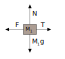
\includegraphics[width=0.4\textwidth]{carrucole.6.pdf}
\end{figure}

\begin{itemize}
\item[$M_1g$] è la \textbf{forza peso} 
\item[$N$] è la \textbf{reazione vincolare} del piano, reazione del piano stesso alla forza peso che impedisce al corpo di cadere attraverso il piano
\item[$T$] è la tensione esercitata dalla fune
\item[$F$] è la \textbf{forza d’attrito dinamico} o \textbf{statico}, a seconda che il corpo sia in quiete o in movimento.
\end{itemize}

\item 
La tensione della fune è pari alla forza esercitata dalla gravità su $M_2$:
\begin{equation*}
T=m_2g
\end{equation*}

Questo valore deve essere equivalente alla forza d'attrito dinamico:

\begin{equation*}
T=f_{max}=\mu_sm_1g
\end{equation*}

\begin{equation*}
\mu_sm_1g=m_2g
\end{equation*}

\begin{equation*}
\mu_s=\frac{m_2}{m_1}
\end{equation*}

\end{enumerate}

Soluzioni degli esercizi multiple choice da pagina \pageref{q_mcmc} \label{s_mcmc}

\begin{enumerate}
\item B
\item C
\item B
\item C
\item B
\item A
\item C
\item C
\item D
\item C
\item B
\item C
\item D
\item C
\item A
\item D
\item D
\item D
\item B
\item C
\item A
\item D
\item C
\item A, B
\item B, C
\end{enumerate}

